\chapter{Implementation}

% organise by features of app/api or by stages?

\section{Overview}

Since the back-end API and front-end mobile app are so tightly connected, implementing them linearly would not be logical as errors between the app and server will not be detected as quickly and requirements of features may change over time. I therefore implemented the two in parallel, normally a feature at a time, so that a working implementation for each subsequent feature was produced at the end of each iteration.

This section splits the implementation into the two sections, API and mobile app, with each discussing the features implemented chronologically.

\section{API}

\subsection{Endpoint Routing}

To set up endpoints on the API to respond to client requests, the popular Express web framework ***ref*** was used. Express's router object determines how the API handles a request to a certain URI with a specific HTTP method.

The main file loaded when a request is made, \texttt{app.js}, specifies the main endpoint for the API and links this endpoint to an Express router. This router specifies the path for each of the main API routes, following the design from Figure \ref{fig:api-routes} in the previous section. Each path contains a router which matches each of the endpoints it serves as well as a controller containing functions which are executed when a router endpoint is matched from a request. An example of how a request to login a user is routed through the API is shown in Figure ***.

\subsection{Authentication}



\subsection{Querying Database}

\subsection{Storing Images} \label{implentation:storing-images}

% mention mongoose populate

\section{Mobile App}

\subsection{Communication with API}

To handle requests from the multiple APIs used within the mobile application, a singleton class \texttt{APIManager} was used that was accessible throughout the app to organise each API call. The main function of \texttt{APIManager} was to abstract the network requests through the HTTP networking library Alamofire ***ref*** -- a more elegant way to handle networking in comparison to Swift's default network tools, providing simple JSON encoding and serialisation as well as response validation.

Alamofire's Router design pattern allowed me to define a complete set of paths, methods and parameters needed for the endpoints of a particular API and hence construct a request with with any HTTP headers as appropriate. The Router was implemented as a protocol containing the necessary fields that needed to be overridden, and each API that needed to be documented in this way adopted this protocol and used an enumeration pattern to define each of the available endpoints for that API. The specific endpoint case for a given API router would then be passed as a parameter to Alamofire's \texttt{request()} method, which would construct and send the HTTP request as necessary.

Finally, an enumeration was created to represent the success or failure response received from the API. Enumeration cases in Swift can contain parameters and so I defined the success response to contain a JSON object that contained the response from the API, constructed in Alamofire's asynchronous request callback. Meanwhile, the failure case contained a Swift error object whose error code and description were populated from the information received from the API. Figure \ref{fig:api-communication} explains in more detail the path of method calls and how data is passed through callbacks when making a network request.

\begin{figure}[hbt]
  \centering
  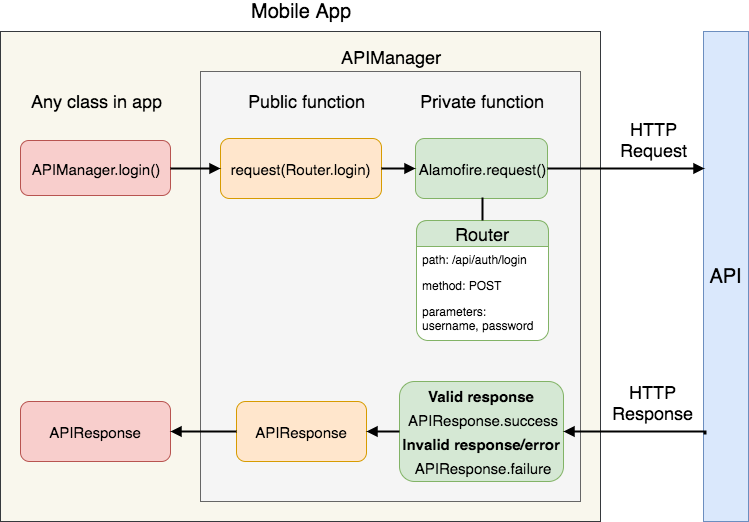
\includegraphics[width=\textwidth]{api-communication}
  \caption{The path of method calls and callbacks used when making a network request within the mobile app, namely logging the user in. The top row of arrows represent method calls being made from the app whilst the bottom row of arrows represent the callbacks for each method once the network response is received.}
  \label{fig:api-communication}
\end{figure}


\subsection{Points of Interest}

\subsection{Gamification} \label{subsection:gamification}

% should this be in mobile app section?

\subsection{Walk invitations}

\section{Challenges}